\chapter{Lecture 28 - Orthogonal Series Expansion}
\label{ch:lec28}
\section{Objectives}
\begin{itemize}
\item Apply separation of variables and solve boundary value problems that have solutions in the form of orthogonal series expansions (other than Fourier series).
\item Show examples with the heat and wave equation.
\end{itemize}
\setcounter{lstannotation}{0} %hack to try and re-set annotation counter.

For some sets of boundary conditions, the solution to the heat equation is an infinite series that is not a Fourier series.  I will argue that, apart from details regarding identifying eigenvalues, the implications of this are not large and will have little impact on how you go about computing the solution.  All of this is most easily clarified with a couple of examples.

\vspace{0.3cm}

\noindent\textbf{Example \#1:}  Consider the boundary value problem below based on the heat equation.
\begin{table}
\begin{tabular}{l l}
$\substack{\text{Governing} \\\text{Equation}}: $& $\frac{\partial u}{\partial t} = \alpha^2 \frac{\partial^2 u}{\partial x^2},  \ \ \alpha>0, \ \ 0<x<1, \ \ t>0$ \\
& \\
$\substack{\text{Boundary} \\ \text{Conditions}}: $& $u(0,t)=0, \ \ u_x(1,t) = -hu(1,t), \ \ h>0, \  t>0$\\
& \\
$\substack{\text{Initial} \\ \text{Conditions}}: $ & $u(x,0) = 1, \ \ 0<x<1 $ \\
\end{tabular}
\end{table}
\begin{marginfigure}
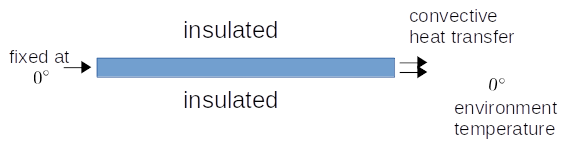
\includegraphics{lec28-ex1-schematic.png}
\caption{Schematic of Example \#1.}
\label{fig:lec28-ex1-schematic}
\end{marginfigure}
A schematic of this problem is shown in Figure \ref{fig:lec28-ex1-schematic}.  On the right end of the domain we have a type 3 boundary condition representing convective heat transfer to an environment maintained at a temperature of 0$^{\circ}$.\marginnote{Note that we have not established any physical units on this system.  If it helps, consider all temperatures given to be in degrees Celsius.}

\newthought{We will solve} this boundary value problem using separation of variables.  Since we have already carried out the separation process for the heat equation numerous times, we will skip ahead and write down the separated equations:
\begin{align*}
u(x,t) &= F(x)G(t) \\
F_{xx} + \lambda F &= 0 \\
G_{t} + \alpha^2 \lambda G &= 0 
\end{align*}
We need to find values of $\lambda$ for which non-trivial solutions to the equations can satisfy the boundary conditions.  Since $F(x)$ is the spatial variable to which the boundary conditions apply, and both boundary conditions are homogeneous, we will focus our attention on the equation for $F(x)$.

\vspace{0.25cm}

\noindent \underline{$\lambda = 0$}:

\begin{align*}
F_{xx} &= 0 \\
F(x) &= c_1x + c_2 \\
F(0) &= c_1(0) + c_2 = 0 \\
\Rightarrow c_2 &= 0 \\
F_x{1} &= c_1 = -hc_1(1) \\
\Rightarrow c_1&= 0
\end{align*}\marginnote[-1.5cm]{Since $h>0$, the only way that $c_1 = -h c_1$ is if $c_1 = 0$.  If $c_1$ were not zero, the last line would imply that $h = -1$ which, since $h>0$, is a contradiction.} So we will rule out $\lambda=0$ since only the trivial solution $F(x)=0$ applies.

\vspace{0.25cm}

\noindent \underline{$\lambda < 0$}:  $\ \ \lambda = -\nu^2, \ \nu>0$.

\begin{align*}
F_{xx} - \nu^2F &= 0 \\
F(x) &= c_1 \cosh{\nu x} + c_2 \sinh{\nu x} \\
F(0) &= c_1(1) + c_2(0) = 0 \\
\Rightarrow c_1 &= 0 \\
F_{x}(1) = \nu c_2 \cosh{\nu} &= -h c_2 \sinh{\nu} \\
\frac{\nu}{h}c_2 &= -c_2\tanh{\nu} \\
\Rightarrow c_2 &= 0
\end{align*}
\begin{marginfigure}
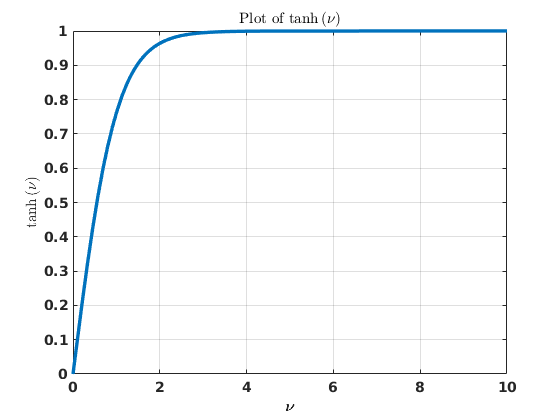
\includegraphics{lec28_plot_of_tanh.png}
\caption{Plot of $\tanh{(\nu)}$.}
\label{fig:lec28-plot-of-tanh}
\end{marginfigure}
Since $\nu>0$ and $h>0$, and, as shown by Figure \ref{fig:lec28-plot-of-tanh} $\tanh{\nu}$ is also positive, $c_2$ must also be equal to zero.\sidenote{By this time, the reader should be getting pretty good at making these kinds of observations.}

\vspace{5.0cm}

\noindent \underline{$\lambda > 0$}: $\ \ \lambda = \nu^2, \ \nu>0$.

\begin{align*}
F_{xx} + \nu^2 F &= 0  \\
F(x) &= c_1 \cos{\nu x} + c_2 \sin{\nu x} \\
F(0) &= c_1 (1) + c_2 (0) = 0 \\
\Rightarrow c_1 &= 0 \\
F_{x}(1) = \nu c_2 \cos{\nu} &= -h c_2 \sin{\nu} \\
c_2 \tan{\nu} &= -\frac{\nu}{h}
\end{align*}
\begin{marginfigure}
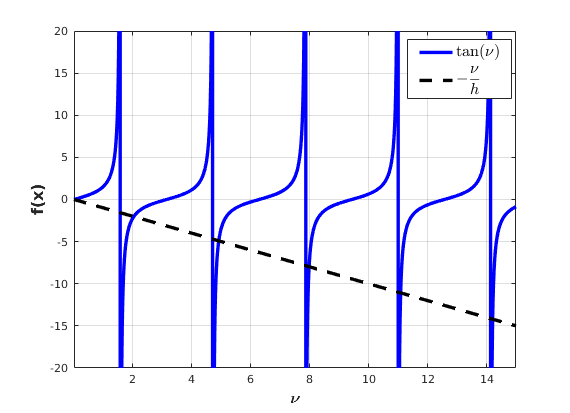
\includegraphics{lec28-fig2.png}
\caption{Plot of $\tan{\nu}$ and $-\sfrac{\nu}{h}$ vs $\nu$ for $h=1$.}
\label{fig:lec28-fig2}
\end{marginfigure}
Of course $c_2 = 0$ would satisfy this condition but we are looking for non-trivial solutions.  We see from Figure \ref{fig:lec28-fig2} that the plot of $\tan{\nu}$ intersects the plot of $-\sfrac{\nu}{h}$ infinitely many times.\sidenote{This is the sort of claim for which a mathematician might reasonably expect a proof but, as engineers, we will simply not provide one.  We know $\tan{\nu}$ is periodic and the pattern will continue indefinitely and the straight line $-\sfrac{\nu}{h}$ will intersect each period no matter the value of $h$ and that will be good enough for us.}  The values of $\nu$ where this happens will be used to find our eigenvalues, $\nu_n^2$, and the eigenfunctions will be $F_n(x) = c_n \sin{\nu_n x}$.  Applying these eigenvalues to our separated equation $G(t)$ gives us:

\begin{align*}
G_{t} + \alpha^2 \nu^2 G &= 0 \\
G_n(t) &= c_3e^{-\left(\alpha \nu_n \right)^2 t}
\end{align*}
and the product solution is:
\begin{equation*}
u(x,t) = \sum\limits_{n=1}^{\infty} c_n \sin{(\nu_n x)}e^{-\left(\alpha \nu_n \right)^2t}
\end{equation*}

\vspace{0.25cm}

\noindent Now we must apply the initial condition:
\begin{equation*}
u(x,0) = \sum\limits_{n=1}^{\infty}c_n \sin{(\nu_n x)}\cancelto{1}{e^{0}} = f(x)
\end{equation*}
On the left side of the equation above we have an infinite series with unknown coefficients $c_n$; on the right side we have a given function $f(x)$.  Our job is to find the values $c_n$ so that the two sides are, in fact, equal.  To do this we will multiply both sides of the equation by our orthogonal functions---$\sin{(\nu_n x)}$---and integrate over the interval $x \in [0,1]$.\sidenote{We should hasten to add---``and weight function''---to this phrase.  It is an important detail that is easy to forget.  When we move on to problems in polar and cylindrical coordinates we will need to be more strict about this. }   At this point we still have not nailed down the numeric values of $\nu_n$ but we \emph{do} know that, since the separated boundary value problem for $F(x)$ from which we obtained $\nu_n$ and $\sin{(\nu_n x)}$ fall within the realm of Sturm-Liouville eigenvalue theory, the eigenfunctions are mutually orthogonal with respect to the weight function, $p(x)$ which, in this case, can be shown to be $p(x)=1$. 

The coefficients are given by:
\begin{equation*}
c_n = \frac{\left(f(x),\sin{(\nu_n x)}\right)}{\left( \sin{(\nu_n x)}, \sin{(\nu_n x)}\right)} = \frac{\int_0^1 f(x) \sin{(\nu x)}\ dx}{\int_0^2 \sin{(\nu x)}^2 \ dx}
\end{equation*}

\newthought{We will use} MATLAB to solve this boundary value problem.  As usual, we will start by clearing out the MATLAB workspace, specify our constants and initial conditions and determine the number of terms to use in our infinite series for $u(x,t)$.

\begin{lstlisting}[name=lec28-ex1, style=myMatlab]
clear
clc
close 'all'

%% Parameters
alpha_sq = 0.1; % thermal diffusivity
h = 10; % convective heat transfer coefficient
L = 1;
f = @(x) 1; % initial condition

N = 25; % number of eigenfunctions


\end{lstlisting}

Next we must find numeric values for $\nu_n$.  To do this, we will observe from Figure \ref{fig:lec28-ex1-schematic} that there is exactly one intersection of $\tan{\nu}$ and $-\sfrac{\nu}{h}$ in the interval $\nu \in [\sfrac{\pi}{2}, \sfrac{3\pi}{2}]$ and another intersection in the interval $\nu \in [\sfrac{3\pi}{2}, \sfrac{5\pi}{2}]$ etcetera.  We keep looking in intervals $[\sfrac{n \pi}{2},\sfrac{(n+2)\pi}{2}], \ \ n=1,3,5,\dots$.  This is done using the MATLAB built-in function \lstinline[style=myMatlab]{fzero()}.
\marginnote[1.0cm]{
\ref{lst:ann28-1-1} \lstinline[style=myMatlab]{fzero()} is a root-finding function so we need to re-formulate $\tan{\nu} = -\sfrac{\nu}{h}$ so a root-finder can get the values of $\nu$.

\vspace{0.25cm}

\ref{lst:ann28-1-2} We do not want to evaluate our function at the ends of the search interval since those correspond to asymptotes of $\tan{x}$.  We move our search boundaries in a little bit to avoid those asymptotes.

}
\begin{lstlisting}[name=lec28-ex1, style=myMatlab]
%% Find the desired number of eigenvalues
ev_fun = @(x) tan(x) + x./h; /*!\annotation{lst:ann28-1-1}!*/

nu = nan(N,1);
delta = 1e-8; /*!\annotation{lst:ann28-1-2}!*/
x0 = [pi/2+delta,3*pi/2-delta];
for i = 1:N
   [x,fval,exit_flag] = fzero(ev_fun,x0); /*!\annotation{lst:ann28-1-3}!*/
   nu(i) = x;
   x0 = x0 + pi;
end
% do some crude error checking
assert(min(diff(nu))>0,...
    'Error! Something is wrong with your eigenvalues!');/*!\annotation{lst:ann28-1-4}!*/

\end{lstlisting}
\noindent \ref{lst:ann28-1-3} In this instance \lstinline[style=myMatlab]{fzero()} has two arguments and returns three values.  The variable \lstinline[style=myMatlab]{ev_fun} is a handle\sidenote{A variable that, when evaluated returns a function is often referred to as a \emph{handle} to the function  This is similar to the variable \lstinline[style=myMatlab]{gca} which can be thought of as a handle to the current axis.} to the function to which we are looking for roots and \lstinline[style=myMatlab]{x0} is the interval where we are searching for the roots.  Of the return arguments: \lstinline[style=myMatlab]{x} is the root; \lstinline[style=myMatlab]{fval} is the numeric value of \lstinline[style=myMatlab]{ev_fun} evaluated at the root \lstinline[style=myMatlab]{x}; and \lstinline[style=myMatlab]{exit_flag} is a value returned by \lstinline[style=myMatlab]{fzero()} to indicate if the function was successful or not.\sidenote{See the documentation for a description of the possible values for \lstinline[style=myMatlab]{exit_flag}.  Several built-in MATLAB functions use this and an \lstinline[style=myMatlab]{exit_flag=1} normally indicates success.  As you can see, we do not check the value of \lstinline[style=myMatlab]{exit_flag} in this script (and we also ignore \lstinline[style=myMatlab]{fval}) but readers are encouraged to make use of this kind of feedback available from MATLAB functions.}

\vspace{0.25cm}

\noindent \ref{lst:ann28-1-4} This is a modest bit of error checking to ensure that, at a minimum, the roots we find are distinct.

\vspace{0.25cm}

\noindent The remainder of the MATLAB script is typical of what we have been doing so far.

\begin{lstlisting}[name=lec28-ex1, style=myMatlab]
%% Construct solution
Fn = @(x,n) sin(nu(n).*x);
Gn = @(t,n) exp(-(nu(n).^2).*alpha_sq.*t); 

u = @(x,t) 0;

for n = 1:N
   ef_mag = integral(@(x) Fn(x,n).*Fn(x,n),0,L); /*!\annotation{lst:ann28-1-5}!*/
   cn = integral(@(x) f(x).*Fn(x,n),0,L)./ef_mag;
   
   u = @(x,t) u(x,t) + cn*Fn(x,n).*Gn(t,n);
end

\end{lstlisting}
\marginnote[-2.0cm]{
\ref{lst:ann28-1-5}  We have not bothered to try and derive a closed-form solution for $\int_0^1 \sin{\left(\nu_n x \right)} \ dx$ so we do it numerically.
}
\begin{marginfigure}
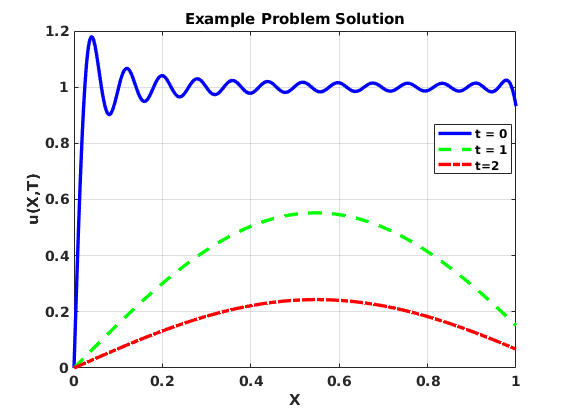
\includegraphics{lec28-ex1-sol.png}
\caption{Solution for Example \#1.}
\label{fig:lec28-ex1-sol}
\end{marginfigure}
The solution for the parameters we have selected, plotted at various times, is shown in Figure \ref{fig:lec28-ex1-sol}

Some questions that you should make sure that you can answer:%\marginnote{
%Rough answers:
%\begin{enumerate}
%\item The steady-state temperature is $u(x,\infty)=0$.  Heat passes out the left and right boundary by conduction on the left and convection on the right.

%\item This is because the initial condition $f(x)=1$ did not satisfy the boundary condition at $x=0$.  As expected, the ``wiggliness'' quickly diffuses away.

%\item If the thermal diffusivity is increased, the temperature progresses towards its steady-state value more quickly.

%\item If the convective heat transfer coefficient is increased, energy is transferred through the right boundary more quickly.  This can most easily be observed by noting the \emph{slope} of the solution at the boundary.  If $h$ is increased, the slope becomes more negative; if $h$ is decreased, the slope becomes less negative.  The limit of $h=0$ corresponds to $u_x(1,t)=0$ which is insulated boundary conditions.


%\end{enumerate}
%}
\begin{enumerate}
\item What is the final steady-state temperature?  Answer: zero since all of the energy from the initial condition is transferred out via the left or right boundaries.

\item Why is the initial condition so ``wiggly''? Answer: because the initial condition does not match the boundary condition at $x=0$ and the discontinuity causes perturbations typical of Fourier series.

\item What happens if $\alpha^2$ is increased or decreased?

\item What happens if $h$ is increased or decreased?
  
\end{enumerate}
\begin{figure}[h!]
\subfloat[]{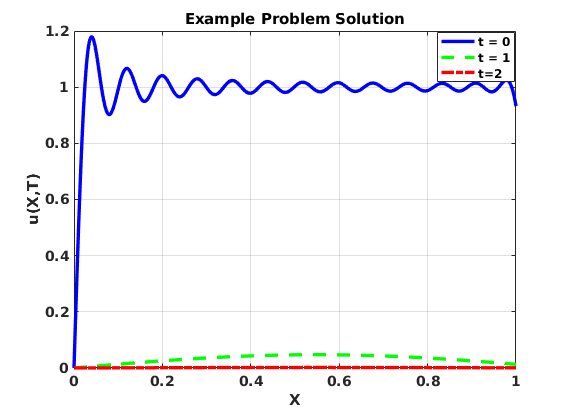
\includegraphics[width=2in]{lec28-ex1-sol-alpha-high.png}}
\subfloat[]{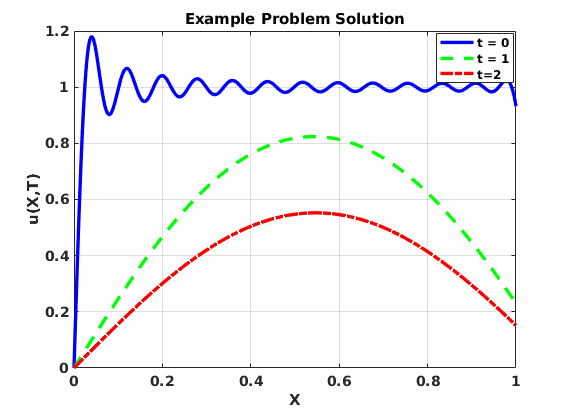
\includegraphics[width=2in]{lec28-ex1-sol-alpha-low.png}} \\
\subfloat[]{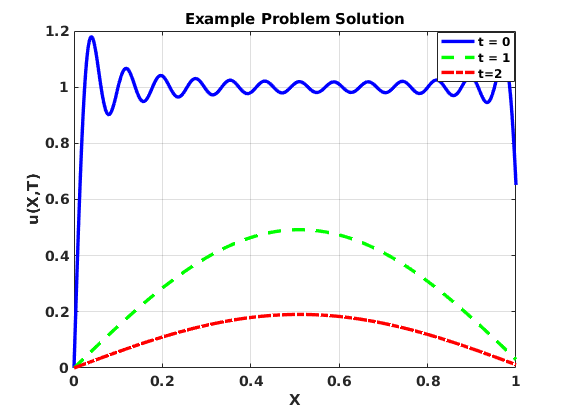
\includegraphics[width=2in]{lec28-ex1-sol-h-high.png}}
\subfloat[]{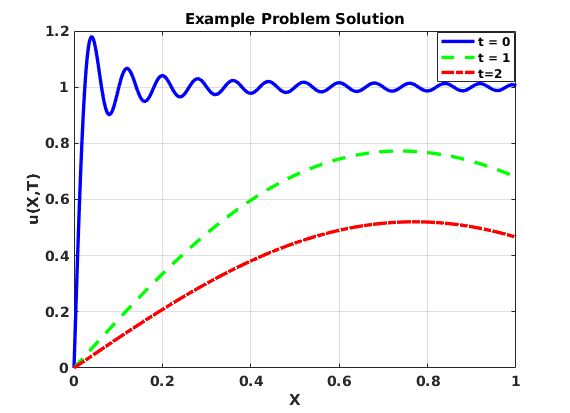
\includegraphics[width=2in]{lec28-ex1-sol-h-low.png}}
\label{fig:lec28-ex1-variations}
\caption{Variations in $\alpha$ and $h$ for example problem.}
\end{figure}
Answers to the last two questions are illustrated in Figure \ref{fig:lec28-ex1-variations}.  Images a) and b) illustrate how the solution changes when thermal diffusivity is increased or decreased, respectively.  Images c) and d) illustrate how the solution changes when the convective heat transfer coefficient, $h$, is increased and decreased.

\vspace{0.5cm}

\noindent\textbf{Example \#2:} The twist angle $\theta(x,t)$ of a torsionally vibrating shaft is given by the wave equation.

\begin{table}[h]
\begin{tabular}{l l}
$\substack{\text{Governing} \\\text{Equation}}: $& $\alpha^2 \frac{\partial^2 \theta}{\partial x^2} =  \frac{\partial^2 \theta}{\partial t^2},  \ \ \alpha>0, \ \ 0<x<1, \ \ t>0$ \\
& \\
$\substack{\text{Boundary} \\ \text{Conditions}}: $& $\theta(0,t)=0, \ \ \theta_x(1,t) = 0, \ \ t>0$\\
& \\
$\substack{\text{Initial} \\ \text{Conditions}}: $ & $\theta(x,0) = x, \ \ \theta_t(x,0) = 0, \ \ 0<x<1 $ \\
\end{tabular}
\end{table}
\begin{marginfigure}
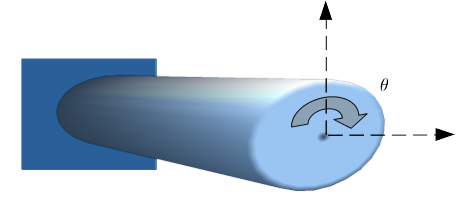
\includegraphics{lec28-ex2-schematic.png}
\caption{Schematic of Example \#2.}
\label{fig:lec28-ex2-schematic}
\end{marginfigure}


\newthought{Of course we} will also use separation of variables for this boundary value problem and, again, since we have already carried out the separation process for the wave equation numerous times, we will again skip ahead and write down the separated equations:

\begin{align*}
\theta(x,t) &= F(x)G(t) \\
F_{xx} + \lambda F &= 0 \\
G_{tt} + \alpha^2 \lambda G &= 0
\end{align*}
We need to find values of $\lambda$ for which non-trivial solutions to the equations can satisfy the boundary conditions.  As with the first example, $F(x)$ is the spatial variable to which the boundary conditions apply and both boundary conditions are homogeneous.  Thus we will again focus our attention on the equation for $F(x)$.

\vspace{0.25cm}

\noindent\underline{$\lambda = 0$}:

\begin{align*}
F_{xx} &= 0 \\
F(x) &= c_1x + c_2 \\
F(0) &= c_1(0) + c_2 = 0 \\
\Rightarrow c_2 &= 0 \\
F_{x}(0) &= c_1 = 0 \\
\Rightarrow c_1 &= 0
\end{align*}
We see that for $\lambda = 0$ only the trivial solution can satisfy the boundary conditions.

\vspace{0.25cm}

\noindent\underline{$\lambda < 0$}: $\ \lambda = \nu^2, \ \nu>0$
\begin{align*}
F_{xx} - \nu^2 F &= 0 \\
F(x) &= c_1 \cosh{\nu x} + c_2 \sinh{\nu x} \\
F(0) &= c_1(1) + c_2(0) = 0 \\
\Rightarrow c_1 &= 0 \\
F_{x}(1) &= \nu c_2 \cosh{\nu} = 0
\end{align*} \marginnote{By this point in time, this analysis may begin to feel quite repetitive.  That is because it \emph{is} repetitive.  Nonetheless, resist the tendency to rush and/or become complacent.  It is worth your while to patiently and carefully work through each of these cases every time.}
For the last conditions, since $\cosh{\nu}$ is always positive for $\nu>0$, $c_2 = 0$ and, again, only the trivial solution can satisfy the boundary conditions.

\vspace{0.25cm}

\noindent\underline{$\lambda > 0$}: $\ \lambda = \nu^2, \ \nu>0$
\begin{align*}
F_{xx} + \nu^2 F &= 0 \\
F(x) &= c_1\cos{\nu x} + c_2 \sin{\nu x} \\
F(0) &= c_1(1) + c_2(0) = 0 \\
\Rightarrow c_1 &= 0 \\
F_{x}(1) &= \nu c_2 \cos{\nu} = 0
\end{align*}
We can satisfy this boundary condition for any value of $c_2$ provided that $\nu$ is a root of $\cos(x)$.  This happens when $\nu$ is an odd-integer multiple of $\sfrac{\pi}{2}$.  Thus:

\begin{align*}
\nu_n &= (2n-1)\frac{\pi}{2}, \ n=1,2,3\dots \\
F_n(x) &= c_n \sin{\nu_n x}
\end{align*} 
The corresponding solution to $G(t)$ is:
\begin{align*}
G_{tt} + \alpha^2 \nu_n^2 G &= 0 \\
G(t) &= a_n \cos{(\alpha \nu_n t)}+b_n\sin{(\alpha \nu_n t)}
\end{align*}
and the product solution is:
\begin{equation*}
u(x,t) = F(x)G(t) = \sum\limits_{n=1}^{\infty} \left[a_n \cos{(\alpha \nu_n t)}+b_n\sin{(\alpha \nu_n t)} \right]\sin{(\nu_n x)}
\end{equation*}

\newthought{To solve for} the remaining constants $a_n$ and $b_n$ we need to apply the initial conditions.
\begin{align*}
u(x,0) &= \sum\limits_{n=1}^{\infty}\left[a_n(1) + b_n(0) \right]\sin{(\nu_n x)} \\
&=\sum\limits_{n=1}^{\infty} a_n \sin{(\nu_n x)} = x
\end{align*}
To solve for $a_n$, we now only need to multiply both sides by our orthogonal function---$\sin{(\nu_n x)}$---and integrate.  The resulting formula for $a_n$ is:\marginnote[1.0cm]{This really \emph{looks} like a Fourier series, but technically it is not since the expansion functions are not $\sin{(\sfrac{n \pi x}{L})}$ or $\cos{(\sfrac{n \pi x}{L})}$.}
\begin{equation*}
a_n = \frac{(x,\sin{(\nu_n x)})}{(\sin{(\nu_nx)},\sin{(\nu_n,x)})} = \frac{\int_{0}^{1}x \sin{(\nu_n x)} \ dx}{\underbrace{\int_0^1 \sin{(\nu_n x)}^2 \ dx}_{\sfrac{1}{2}}}
\end{equation*}

\vspace{0.25cm}

\noindent The other boundary condition is applied to get $b_n$:
\begin{align*}
u_t(x,0) &= \sum\limits_{n=1}^{\infty} \left[-\alpha \nu_n a_n (0) + \alpha \nu_n b_n(1)\right]\sin{(\nu_n x)} = 0 \\
\Rightarrow b_n &= 0, \ \ n=1,2,3\dots
\end{align*}

\noindent In summary, the solution is:
\begin{align*}
u(x,t) &= \sum\limits_{n=1}^{\infty} a_n \cos{(\alpha \nu_n t)}\sin{(\nu_n x)} \\
a_n &= 2 \int_0^1 x \sin{(\nu_n x)} \ dx
\end{align*}

\newthought{The MATLAB code} to construct and visualize the solution for this problem is shown in the listing below.

\begin{lstlisting}[name=lec28-ex2, style=myMatlab]
clear
clc
close 'all'

%% Parameters
alpha_sq = 5;
L = 1;

N = 30;

nu = @(n) (2*n-1)*pi/2;
Fn = @(x,n) sin(nu(n).*x);
Gn = @(t,n) cos(alpha_sq*nu(n).*t);
f = @(x) x; % initial displacement
u = @(x,t) 0; % initial velocity

for n = 1:N
   ef_mag = integral(@(x) Fn(x,n).^2,0,L);
   an = integral(@(x) f(x).*Fn(x,n),0,L)./ef_mag;
   
   u = @(x,t) u(x,t) + an.*Fn(x,n).*Gn(t,n);
end

%% Plot the solution
Nx = 1000;
X = linspace(0,L,Nx);

Tmax = 5;
Nt = 50;
T = linspace(0,Tmax,Nt);

figure(2)
for t = 1:Nt
    plot(X,u(X,T(t)),'-b','linewidth',3);
    title_str = sprintf('Lecture 28 Example 2, t = %g ',T(t));
    title(title_str,'fontsize',16,'fontweight','bold');
    xlabel('X','fontsize',14,'fontweight','bold');
    ylabel('U(X,T) Angular Displacement', 'fontsize',14,...
        'fontweight','bold');
    grid on
    set(gca,'fontsize',12,'fontweight','bold');
    axis([0 L -L L]);
    pause(Tmax/(Nt-1));    
end
\end{lstlisting}

